\chapter{DiscoverySpace: Suggesting Actions in Complex Software}
\label{chapter:discoveryspace}
\begin{quote}
When using complex software for the first time, sometimes even video assistance can be too overwhelming. RePlay and ReMap found that people don't always know what help to search for to achieve their goal, and novices may not even know what goals are possible. LiveClips proposed contextual examples to help users explore potential outcomes, but it does not help them \textit{achieve} these outcomes. Even when following tutorials, novices often get lost in the many steps required to achieve their goals. To address these challenges, this chapter introduces \textit{Discovery\-Space}, a contextual panel for Adobe Photoshop that suggests action macros to apply to photographs. Discovery\-Space harvests these one-click actions from the online Photoshop user community. A between-subjects study indicated that action suggestions may help novices maintain confidence, accomplish tasks, and discover features. This work demonstrates how interfaces can leverage user-generated content to help novices achieve expert-level outcomes in complex software.
\end{quote}

\section{Introduction}
Software tends to accrue features and complexity over time [1,20,23,24]. This bloat creates a steep learning curve in four ways: First, novice users often have a different vocabulary than the application [1], making it difficult to locate desired features. Second, while online tutorials abound, they can be hard to follow and users must interpret and adapt them to suit their situation and goals [14]. Third, software often provides several strategies for accomplishing similar tasks. Some are faster, easier, or more effective than others, and it can be difficult to identify which these are. Finally, users are typically only aware of a small percentage of software features [24]; there may be potential results they could achieve but do not think to try.

Accomplishing one's goal with software generally requires composing multiple commands into a sequence. The bur-den is on the user to know which tools to combine and how to apply them. This paper aims to reduce the execution gap between users' high-level task goals and the low-level steps needed to achieve them, by suggesting action macros. These aggregated action suggestions move the user's focus from individual \textit{operations} to human-understandable, goal-driven \textit{activities} [21].

We investigate the efficacy of action suggestions through Discovery\-Space, a recommendation interface for action macros recorded by the user community. Action macros encapsulate a sequence of operations that is executed as a batch. The Discovery\-Space prototype is a Photoshop panel comprising action macros that can be applied in one click for quick and easy exploration. We hypothesize that action suggestions help users get started in complex applications by enabling them to easily explore creative possibilities and achieve quick results.

This paper contributes a prototype action suggestion system, Discovery\-Space, and the results of a preliminary experiment to examine its efficacy. This between-subjects study found that action suggestions may help prevent novices from losing confidence in their abilities, and help users to accomplish tasks and discover new features. This paper also proposes design guidelines for a suggestion interface based on these observations and results.

\section{Related Work: Helping Novices Use Software}
The literature offers several strategies for helping novices effectively use software: some focus on high-level tasks, others on lower-level tool use. Figure 1 describes how our approach relates to this prior work. 

\subsection{Interactive Tutorials Provide Step-by-step Guidance}
Online tutorials are a popular resource for users of complex software. However, they present difficulties such as switching back and forth between the browser and the application, and mapping screenshots or videos of the application to the user's own version [14,29]. Interactive tutorials address these challenges by guiding users step-by-step through hands-on example tasks inside the target application [14,17,29]. Such tutorials can even be generated automatically as a user demonstrates them [10]. However, there are still far more user goals than authored tutorials, and automatically making static tutorials interactive remains a challenge [8,18]. In addition, users must translate between their own goals and the available tutorials.

Tutorials teach users to use applications step-by-step. Other systems focus on speeding up holistic tasks rather than teaching individual steps. For example, TappCloud introduced ``semi-automated'' tutorials that can be applied in one step, like macros, but also allow for the user to interact with each step if desired [18]. However, TappCloud users do not interact directly with the application's tools, but instead with visual previews of different parameter settings. Discovery\-Space also focuses on smoothing the execution process rather than helping users learn the application.

\subsubsection{Adaptively Disclosing Interface Functionality}
Adaptive interfaces initially provide a simplified interface and progressively disclose additional features either automatically [9,23,26], or by allowing users to move between predefined interface stages [6,19,23,30]. Adaptive interfaces are most successful when they are controllable, predictable, efficient, and promote feature discovery [24,31]. However, achieving all of these is a well-recognized challenge [7,23]. Interfaces that disclose or move features automatically based on user behaviour (\textit{e.g.}, adaptive toolbars in Microsoft Word [9]) can improve efficiency, but often feel unpredictable, uncontrollable, and distracting [9,26,31].

Photoshop Elements is an example of an interface with predefined stages: quick, guided and expert. Users can choose a mode appropriate for their task and skill level, such as quick mode for easily accomplishing basic edits. However, because each mode is associated with a different level of complexity, the interface layout and grouping of tools differs between the modes, making it difficult to transition from one to another.

Adaptive interfaces have mainly focused on task completion efficiency as the performance metric [9,19]. However, for open-ended creative tasks, speed is often less important than discoverability and final quality. Progressive disclosure impedes discoverability by hiding interface elements [7]. Discovery\-Space addresses discoverability by suggesting actions users may not have known to be possible.

\subsection{Command Suggestions and Previews}
CommunityCommands introduced the idea that recommending commands to users can improve an application's discoverability [20,22]. It uses collaborative filtering to suggest AutoCAD commands that are unknown to the current user but frequently used by others in tandem with the current user's frequent commands. Though command recommendations improve discoverability of new features [20], suggesting tool-level commands still requires the user to compose and apply them. Inspired by this, Discovery-Space uses suggestions to promote exploration and discovery, but in the form of task-level actions rather than tool-level commands. 

Previewing results helps users predict what a command will do without having to execute it first. Side Views demonstrated that previews are especially valuable when shown as multiples with different parameter settings [32]. Building on this, suggesting and previewing alternative courses of action provides users with ideas they may not have considered, speeds the iterative design loop, and shows the con-textual effects of changes. Inspired by DesignScape's suggestion interface for graphic design layouts [25], Discovery¬-Space provides both minor (refinement) and major (radical) suggestions.

Popular recommendation algorithms, like collaborative and content-based filtering [27], rely on users' behaviour and preferences as input. For suggestions within a user inter-face, the user often begins with a document, 3D model, or image. Suggestions should be content-dependent, since different documents will benefit from different types of operations. For example, DesignScape generates layout suggestions by altering existing elements in the document [25]. Since visual editing operations can have vastly different outcomes on different images [2], it is important to suggest effects that make sense for the content in question. Our algorithm therefore takes into account the content of the image to produce relevant suggestions.

\subsection{Natural Language Search}
To help users find functionality, applications like CommandSpace integrate search directly into the interface [1]. Natural language search reduces the gap between user language and application language [1]. Inspired by this work, Discovery\-Space includes search functionality in addition to automatic suggestions. Discovery\-Space also provides simple faceted browsing, the ability to refine a collection based on metadata characteristics [15]. Facets are especially beneficial for ``exploratory searchers'' who tend to have only a partial idea of what they are looking for [12]. Faceted search and browsing were designed for information retrieval tasks; Discovery\-Space extends this underlying idea to executable \textit{actions}.

\section{What kind of help do novices need?}
To unearth novice-expert differences in creative software usage strategies, we conducted nine 30-minute sessions in which three expert photo editors helped seven novices edit their photos using Adobe Photoshop and Lightroom. Each session included one novice and one expert (\autoref{fig:discoveryspace_obs}). The novice described their goals while the expert controlled the program and communicated with the novice to help achieve them. One-on-one tutoring like these pair discussions is highly effective for teaching [3], and consequently a valuable model for what software could achieve. We observed these interactions to see what novices asked, how experts translated these requests into image editing operations, and whether there were novice-expert language differences or communication challenges. Our intuition is that good software should enable novices to solve challenges like these for themselves. After all the sessions, we reviewed our notes and looked for recurring behaviour patterns. The following four insights were most prominent:
\begin{enumerate}
    \item Novices often did not know what they wanted to do with a photo, and could not picture how it might be improved. In these cases, the experts would provide their own suggestions to get things started.
    \item Novices had very high-level goals (\textit{e.g.}, ``I want to make this person stand out more''), and often did not know what tools or techniques were needed to accomplish them. Experts were able to translate these goals into concrete operations.
    \item A common way to show a novice what an effect will do was to execute it on the photo and compare the result with the original photo, sometimes exaggerating the effect to illustrate the difference before dialing it back down. Novices were sometimes hesitant about an expert's suggestion, but after seeing its effect on the image would become more excited about it.
    \item Novices appreciated both suggestions that were relevant to their goals, \textit{and} suggestions for different effects they would not have otherwise thought of.
\end{enumerate}

\begin{figure}
\centering
  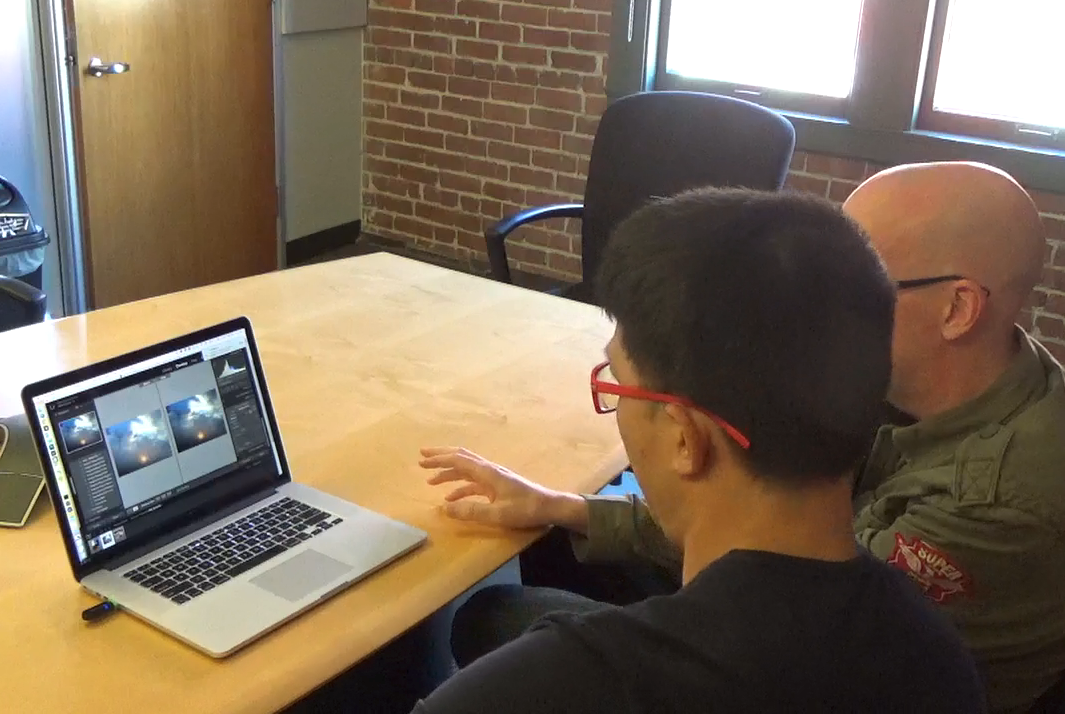
\includegraphics[width=0.6\textwidth]{discoveryspace/figures/obs.png}
  \caption{A novice-expert session. The expert (right) compares the edited photo with the original to illustrate what the edits did.}~\label{fig:discoveryspace_obs}
\end{figure}

\section{Design Goals}
Presenting suggestions relevant to the user's goal can help them accomplish it, as the experts did. Presenting suggestions the user might not have otherwise thought of can help them to discover what is possible and achieve creative results. Combining these insights with prior recommendation research (\textit{e.g.} [12,13,15,20]), we developed five main \textbf{design goals} for suggestion interfaces:
\begin{enumerate}
    \item \textit{Help users get started}: Make suggestions available as soon as the user begins a task. A frequent observation throughout our formative study and prototyping process was that users often did not know where to start in Photoshop.
    \item \textit{Use human language}: Allow users to search using goal terminology, and describe suggestions in a language novices can understand by including a descriptive non-technical title for each. This reflects the growing popularity of natural language or ``semantic'' search [13].
    \item \textit{Show previews} of what a suggestion does, and allow users to easily compare before and after, for example as in Side Views [32].
    \item \textit{Offer faceted browsing} in addition to search to help users explore. This is a well-documented concept in the information retrieval literature (\textit{e.g.}, [12,15,33]), and we believe it to be applicable to software applications as well.
    \item \textit{Suggestions should be relevant} to the user's current task, but should also alert the user to new or unknown possibilities. CommunityCommands users were found to prefer ``contextual'' suggestions related to their short-term history [20], and users of complex software often desire the ability to discover new features [24].
\end{enumerate}

We iterated on the Discovery\-Space design based on feed-back from users with varying levels of Photoshop proficiency. Because Discovery\-Space harvested actions from multiple online sources, they had widely varying amounts of user interaction: some automatically applied effects, while others paused at key points with dialogs for user interaction. We removed such pauses and dialogs when present because they tended to lack sufficient accompanying explanation, and therefore confused some non-expert pilot testers. Users often desired basic adjustments such as brightness/contrast, exposure, and saturation. The actions in our collection generally comprised several steps rather than just one, and so did not include many of these basic edits. We manually created 11 actions for these basic adjustments, which would simply initialize the values to auto, and leave the sliders visible for the user to adjust as they wish.
\section{DiscoverySpace: Action Suggestions}
This section describes the Discovery\-Space interface (\autoref{fig:discoveryspace_interface}) and its keyword-based suggestion algorithm.

\begin{figure}[b!]
\centering
  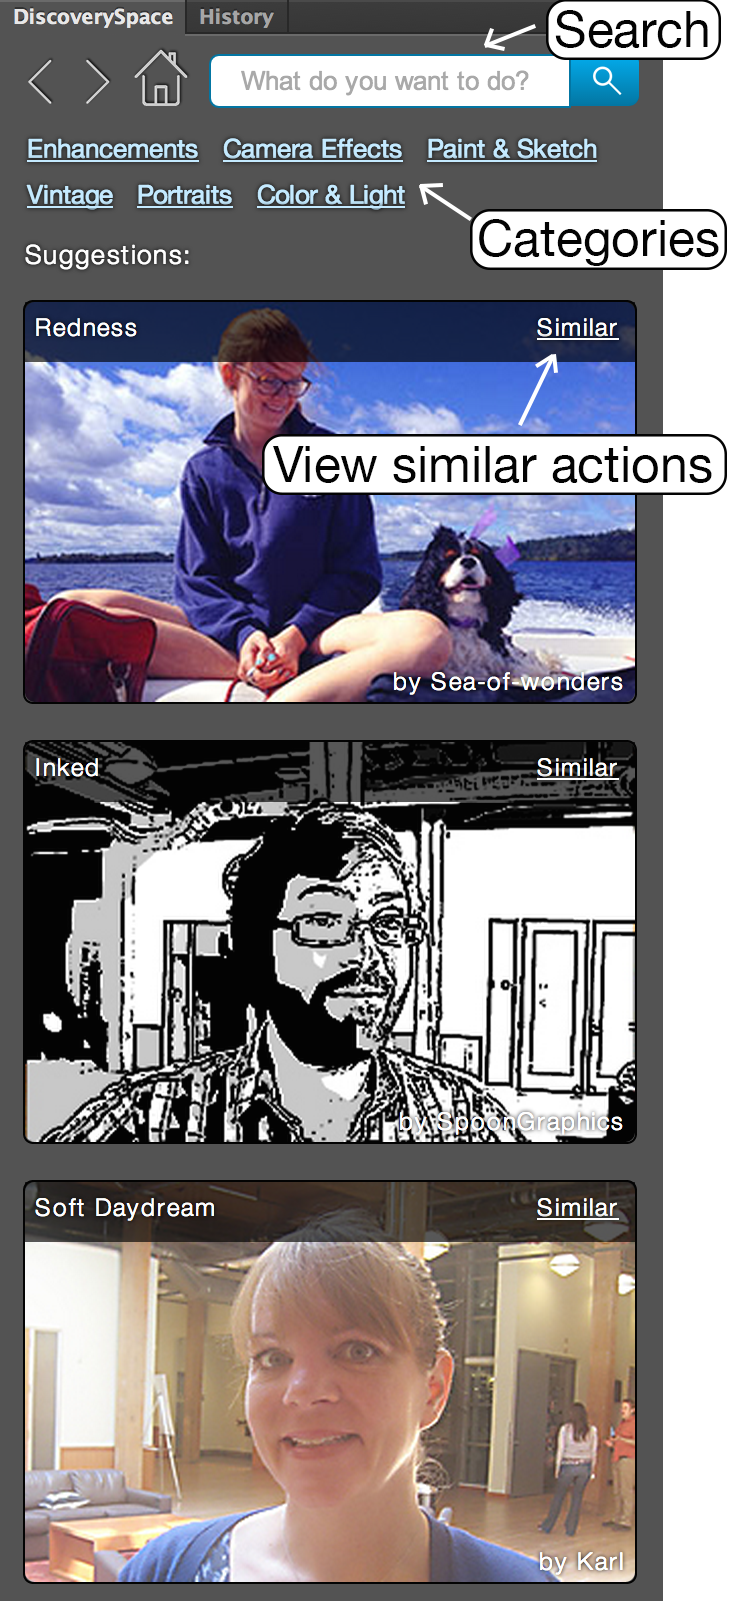
\includegraphics[width=0.35\textwidth]{discoveryspace/figures/discoveryspace_with_labels.png}
  \caption{DiscoverySpace as a panel in Photoshop. Users can apply a suggested action by clicking on its image.}~\label{fig:discoveryspace_interface}
\end{figure}

\subsection{User Experience}
When a user first opens a photo, Discovery\-Space prompts them to enter a goal and select features their image contains from a list (\textit{e.g.} ``contains people'', ``outdoor''). Next, the Discovery\-Space home page appears, containing a search bar, category buttons, and suggested effects (\autoref{fig:discoveryspace_interface}). Each suggestion is displayed by showing the effect applied to an example image with appropriate content. For example, the image for a ``skin smoothing'' effect is of a close-up face. The user can mouse over the image to compare \textit{before} and \textit{after}. Clicking a suggestion applies that action to the photo. As given, the user has no control over the settings for each step of the action; they can see the sequence of steps that was done after applying it by opening the History panel (\autoref{fig:discoveryspace_history}), but cannot step through it or adjust the parameters of individual operations. These actions are therefore intended to allow users to quickly achieve an effect without needing to manually complete all of the intermediate steps. The user can easily undo or redo the effect once it has been applied. If the user scrolls down on the main page, more suggestions appear. To browse suggested effects in a specific category, the user can click a category button. To search the corpus of effects, the user can enter a query in the search bar. The user can also browse effects that are similar to a selected effect by clicking the ``\textit{Similar}'' button on the effect. 

\begin{figure}[b!]
\centering
  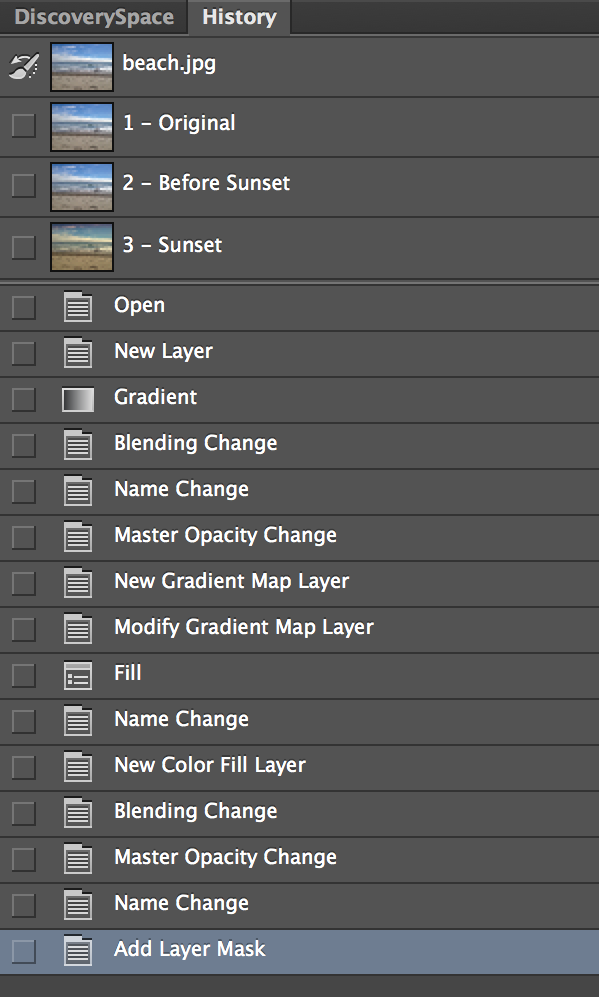
\includegraphics[width=0.35\textwidth]{discoveryspace/figures/history.png}
  \caption{In the History panel, users can review the operations an action has performed.}~\label{fig:discoveryspace_history}
\end{figure}

\subsection{Implementation}
Discovery\-Space is a Photoshop extension panel, written in HTML, Javascript, and Adobe ExtendScript. It retrieves a manually-curated corpus of 115 actions stored on an Amazon S3 server, providing the flexibility to update the actions to reflect popular trends. We manually defined the action categories by reviewing and clustering free actions found online. We created the corpus by downloading 2-3 actions from each subcategory. Paid actions could be added in the future by allowing users the option to pay for effects from within the panel. Discovery\-Space automatically augments search queries with synonyms to maximize the number of relevant results.

\subsection{Keyword-based Recommendations}
Discovery\-Space recommendations take the user's photo as input (\autoref{fig:discoveryspace_rec_alg}). Each action has been assigned a number of descriptive keywords. When opening a new photo, users must select features that describe the image; image analysis could automate this step in the future. We map the selected features to potentially relevant keywords, and assign each action a weight based on the number of matching keywords.

\begin{figure}[b!]
\centering
  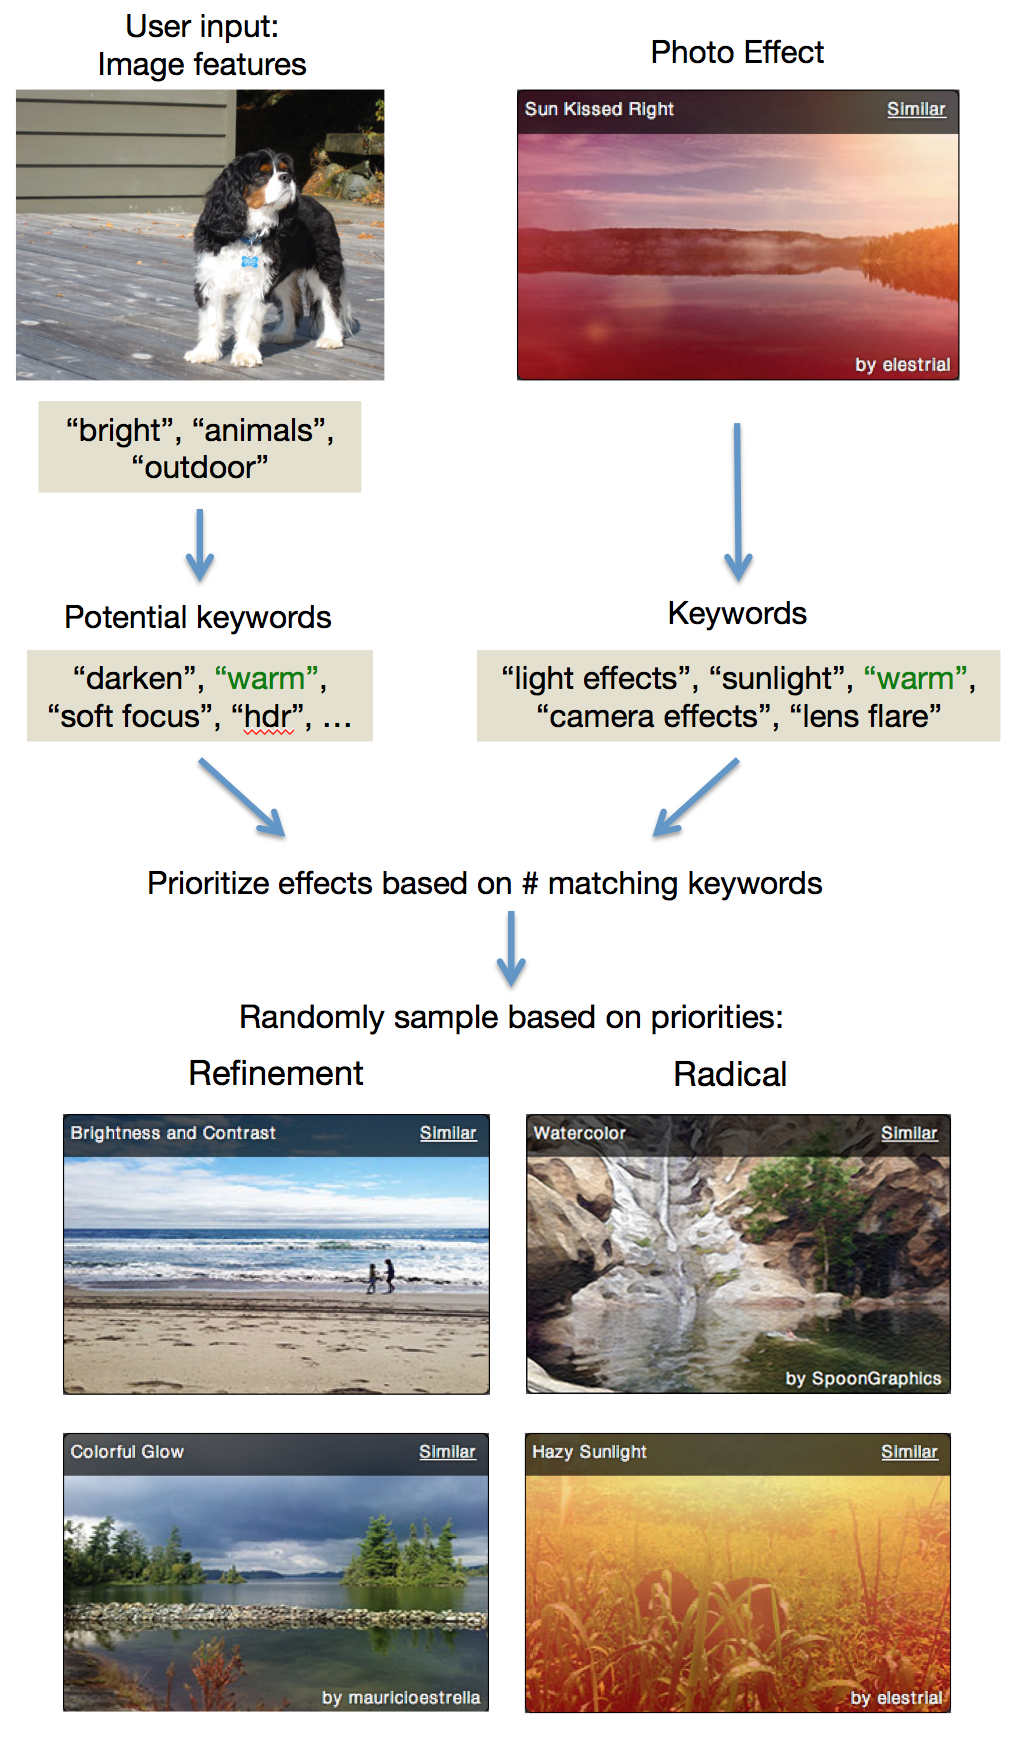
\includegraphics[width=0.6\textwidth]{discoveryspace/figures/rec_alg_new.png}
  \caption{An overview of our keyword-based recommendation algorithm. User-selected image features are mapped to keywords and matched against the keywords for each action in the corpus.}~\label{fig:discoveryspace_rec_alg}
\end{figure}

To select and present suggestions, our algorithm randomly samples from the collection of actions based on these weights: actions with a larger weight have a higher probability of being selected. The randomness encourages discovery by presenting new suggestions when the user refreshes the page. Each action has also been manually classified as either \textit{refinement} or \textit{radical}. An action is deemed \textit{radical} if it produces a drastic effect, does not necessarily maintain realism, and/or takes multiple steps to accomplish. Examples include painting effects, HDR, replicating old cameras, and drastic color effects. An action is deemed a \textit{refinement} if it involves a small adjustment that is meant to improve the photo while maintaining realism, or could be accomplished in one step. Examples include brightening, softening skin, sharpening, and slight color casts. We prefer that both types of effects are suggested, to promote variety in the options. To ensure this, we run the prioritization algorithm separately on the two collections of actions, and then, for every four actions that are suggested, we sample two from the refinement pool and two from the radical pool. This is because on a 27-inch desktop display, Discovery\-Space in its default position shows four suggestions at a time.

\section{Study}
To investigate the efficacy of action suggestions, we conducted a between-subjects experiment in which participants edited their own photos in Photoshop. In the experimental condition, subjects had access to Discovery\-Space; in the control condition they did not. We hypothesized that participants exposed to the suggestions in Discovery\-Space would find the editing process easier, feel more creative, and become more confident using Photoshop. 

\subsection{Method}
To sign up, participants completed a brief initial survey about their Photoshop experience. Participants were then scheduled for a 30-minute session and assigned to one of two conditions: participants in the Discovery\-Space condition used Photoshop with the Discovery\-Space panel open, and participants in the Control condition used Photoshop with a blank panel that instructed them to save their photo when finished (\autoref{fig:discoveryspace_exp_interface}). The study held constant the length of the session (30 minutes), the number of photos edited (two), the questions participants answered when opening and closing a photo, and the availability of a web browser (yes). 

Each session comprised the following steps: consent form, background questions, edit first photo, edit second photo, short interview, and final online survey. The background questions allowed participants to elaborate on their initial survey responses regarding their prior experience with Photoshop and photo editing. Participants were instructed to bring one photo containing at least one person, and one photo without people, to ensure some consistency across participants' photos. The editing order of the two photos was randomly assigned with balancing in each condition. We chose to allow participants to bring their own photos, rather than provide sample photos, so that participants would be more likely to come up with their own goals for their photos, and would be motivated to do a good job. 

\begin{figure}
\centering
  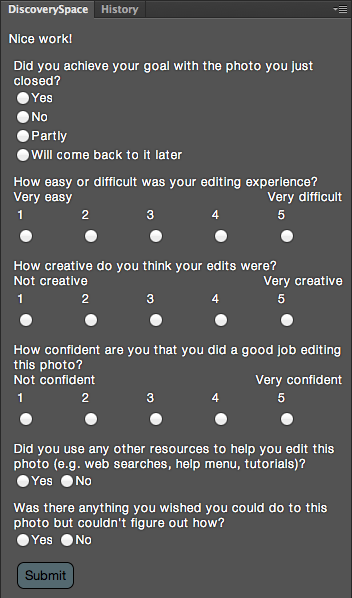
\includegraphics[width=0.6\textwidth]{discoveryspace/figures/close_questions.png}
  \caption{Questions answered by participants after editing each photo. The measure for ``How confident are you that you did a good job editing this photo?'' is referred to as ``confidence about performance'' in the Results.}~\label{fig:discoveryspace_close}
\end{figure}

In both conditions, upon opening a photo, the study panel prompted the user to describe their goal for the photo and select its image features. The panel also prompted the user to answer a few questions about their editing experience every time a photo was closed (\autoref{fig:discoveryspace_close}). The panel was in a prominent location and the participants were made aware of it by the experimenter. The task was open-ended: participants could define their goal however they wanted and were simply instructed to work until they were satisfied (or until time ran out).  We used an open-ended task as opposed to a more directed one because participants would be more likely to perform as they would in a real-world setting when working on personally meaningful tasks. In the Discovery\-Space condition, participants were given a quick overview of the Discovery\-Space interface and were shown what each button in the panel did, so that time would not be wasted figuring out how to use the interface. The History panel was located behind Discovery\-Space, and was only visible when clicked on. Participants in the Discovery\-Space condition were shown the History panel only if they asked explicitly how to go back in time by more than one action. 

In both conditions, a web browser was open on the Google home page just behind Photoshop; participants were told they could use it at any time. This was included to reflect the ready availability of web resources in creative workflows. A short interview and final survey took place in the last five minutes of the session. It comprised follow-up questions on the participant's overall editing experience and their perceived difficulties. 

\subsection{Participants}
28 students were recruited from four undergraduate classes at a Southern California university (one photography class, three design classes). None of these classes provided formal training in Photoshop, though many participants had experience with other photo editing software and/or basic photography principles. Stratified randomization was used to balance gender and Photoshop expertise across conditions. Expertise with Photoshop was measured as follows: in the initial survey, participants were asked to rate their skill level with Photoshop from 1 to 5, and their amount of experience with Photoshop from 1 to 5. The answers to these two questions were added together to produce a score between 2 and 10, and participants were grouped according to their score into Beginner (2-4), Intermediate (5-7) and Expert (8-10). See \autoref{table:ds_participants} for the distribution of participants' expertise and gender. 15 participants were assigned to the Discovery\-Space condition, and 13 to the Control condition (the uneven balance was due to the stratified randomization).

\begin{table}[]
\centering
\begin{tabular}{l|lll}
 & Female & Male & \textbf{Total} \\ \hline
Beginner & 6 & 5 & \textbf{11} \\
Intermediate & 3 & 9 & \textbf{12} \\
Expert & 1 & 4 & \textbf{5} \\
\textbf{Total} & \textbf{10} & \textbf{18} & \textbf{28}
\end{tabular}
\caption{Participants' gender and Photoshop expertise. ALL TABLE CAPTIONS MUST GO ABOVE}~\label{table:ds_participants}
\end{table}

\begin{figure}
\centering
  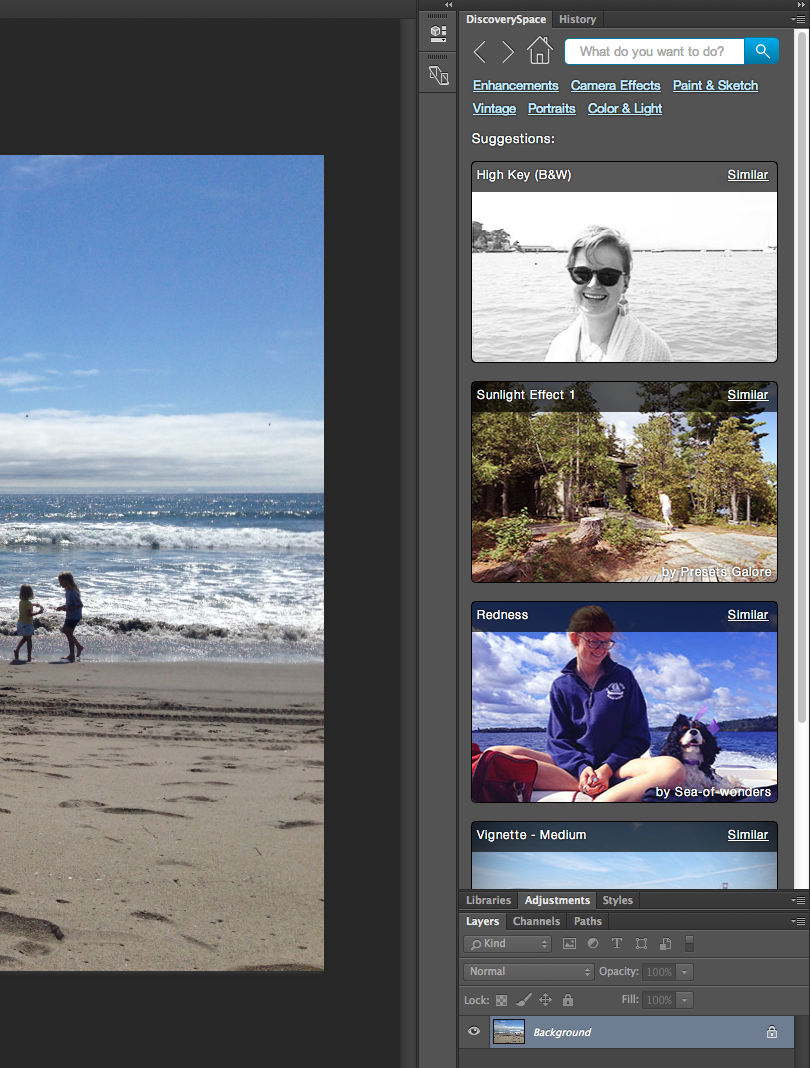
\includegraphics[width=0.4\textwidth]{discoveryspace/figures/experiment-DS.png}
  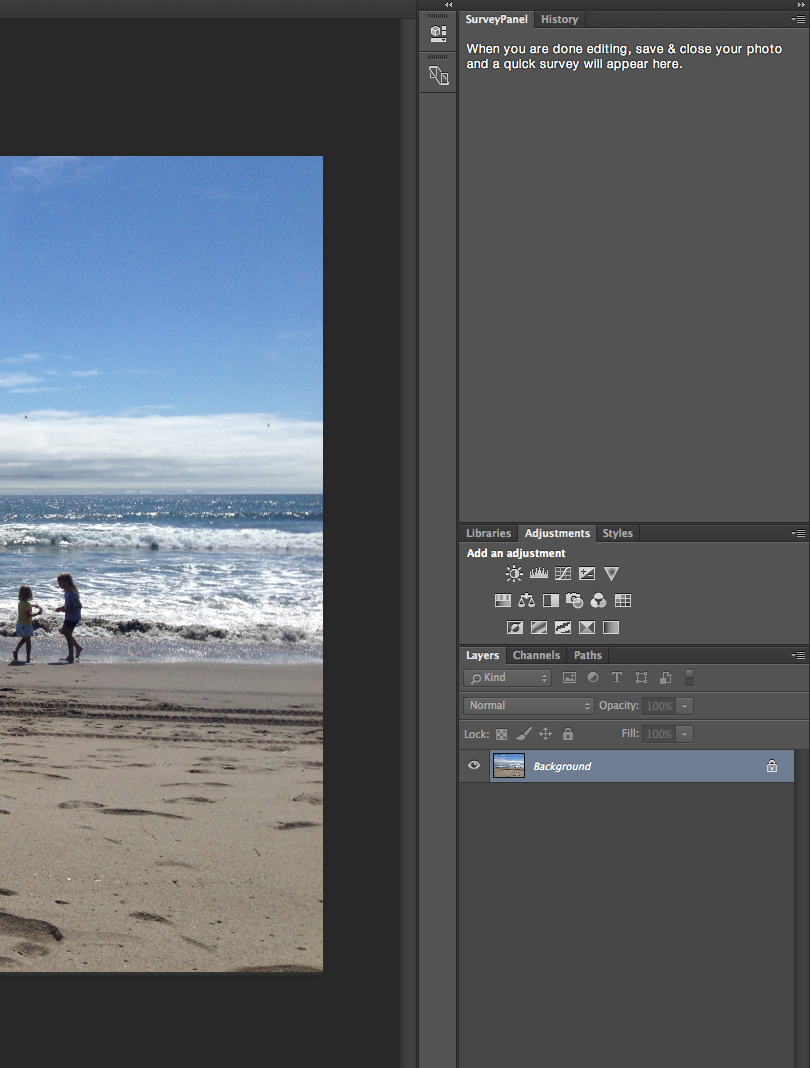
\includegraphics[width=0.4\textwidth]{discoveryspace/figures/experiment-C.png}
  \caption{Photoshop as it appeared in the DiscoverySpace condition (left) and Control condition (right).}~\label{fig:discoveryspace_exp_interface}
\end{figure}

\subsection{Measures}
Both surveys asked participants to rate their Photoshop confidence by answering two questions: ``How confident are you with your ability to edit photos in Photoshop? (1-5)'' and ``How confident are you that you can achieve your goals in Photoshop? (1-5)''. We measured change in confidence as the difference between the sum of both responses (between 2 and 10) in the final survey and the initial survey. For each of the three Likert-scale questions answered after every photo (\autoref{fig:discoveryspace_close}), we added the responses from both photos to obtain one score between 2 and 10 for each participant ($N = 28$). For the questions with yes/no answers, we considered each photo separately ($N = 56$ as each participant edited two photos). We also recorded the number of Photoshop tools used (not including those from Discovery\-Space) and all clicks and pages loaded in Discovery\-Space.

\subsection{Results}
For the numerical measures, we used analysis of variance to analyze Condition, Expertise, and their interaction. For yes/no measures, we used logistic regression with the same variables. 

\subsubsection{Participant Goals}
As expected with such an open-ended task, there was a large variety of participant goals. The most frequent goals focused on color/brightness (\textit{e.g.}, ``correct exposure and color balance'' or ``experiment with color''), or a particular emotional effect (\textit{e.g.}, ``make it surreal looking'' or ``give a lonely, solemn feel''). As expected, participants more often (72\% of the time) used non-technical terms to describe their goals rather than photography-specific terms such as ``saturation'' and ``sharpness''. This was most prominent among Beginners and Intermediates.

\subsubsection{Quantitative Results}
Beginner participants in particular were significantly more likely to lose confidence in the Control condition ($M = -2.0$) and gain confidence in the Discovery\-Space condition ($M = 0.5$), $t(22) = -2.16, p = 0.04$ (\autoref{fig:discoveryspace_confidence}). Across all Expertise levels, Discovery\-Space had only a marginal effect on participants' confidence: the confidence of Control participants decreased ($M = -0.77$) while the confidence of Discovery\-Space participants increased ($M = 0.27$), but this was not significant, $F(1, 22) = 2.97, p = 0.10$. No effect was found for Expertise. 

\begin{figure}
\centering
  \includegraphics[width=0.6\textwidth]{discoveryspace/figures/confidence-new.png}
  \caption{Confidence of Beginner Control participants decreased while confidence of Beginner Discovery\-Space participants increased. Error bars show 1 standard error from the mean. Note that due to small sample sizes in the sub-conditions, this is intended only as a descriptive illustration.}~\label{fig:discoveryspace_confidence}
\end{figure}

\begin{table}[]
\centering
\begin{tabular}{l|l|l|l}
 & DiscoverySpace & Control & $p$ \\ \hline
\textbf{Total confidence change (-8 – 8)} & \textbf{0.27} & \textbf{-0.77} & \textbf{0.10} \\
\textbf{Couldn’t figure something out = yes} & \textbf{50\%} & \textbf{80\%} & \textbf{0.02} \\
Achieved goal = yes & 47\% & 31\% & 0.72 \\
Used web browser & 33\% & 54\% & 0.26 \\
Difficulty (2 – 10) & 5.3 & 6.0 & 0.37 \\
Creativity (2 – 10) & 4.5 & 4.1 & 0.86 \\
Confidence about performance (2 – 10) & 5.9 & 5.2 & 0.68 \\
\# Photoshop tools used & 15 & 20 & 0.38
\end{tabular}
\caption{Summary of mean values for measures compared between conditions. Discovery\-Space participants had marginally \textit{higher} confidence change (this effect was significant within the Beginner group), and stated they could not figure something out \textit{less often} than Control participants.}~\label{table:ds_results}
\end{table}

Discovery\-Space participants were significantly less likely to state that there was something they couldn't figure out ($M = 50\%$) than Control participants ($M = 80\%$), $\chi^2(1) = 5.52, p = 0.02$. 

All measures compared between conditions are summarized in \autoref{table:ds_results}. Responses to many of the post-editing questions varied widely. Within the Beginner group, Discovery\-Space participants rated difficulty as marginally but not significantly lower ($M = 5.3$) than Control participants ($M = 6.8$), $t(22) = 1.62, p = 0.12$. 

Across both conditions, Experts rated difficulty significantly lower ($M = 4.4$) when compared against Intermediates ($M = 5.8$) and Beginners ($M = 6.0$) together, $t(22) = -2.14, p = 0.04$. Experts also used significantly more tools ($M = 26$) than Intermediates ($M = 16$) and Beginners ($M = 16$), $t(22) = 2.37, p = 0.03$. In the Discovery\-Space condition, 51\% of the actions used were radical and 49\% were refinement, which suggests both types of actions were useful.

Overall, there was a strong negative correlation between difficulty and confidence about performance, $r(28) = -.70, p < .0001$. Interestingly, there was also a strong positive correlation between creativity and confidence about performance, $r(28) = .67, p < .0001$.  This effect seems to hold most strongly for Beginners, as the correlation was weaker for Intermediates and Experts only, $r(17) = 0.48, p = 0.05$. Further exploration revealed that using the web was negatively correlated with achieving one's goal, $\chi^2(1) = 8.09, p = .005$, and positively correlated with having trouble figuring something out, $\chi^2(1) = 6.93, p = 0.01$.

Preliminary analyses found no effects for type of class (photography vs. design), so this was excluded from further analyses. Gender was confounded with Expertise (\autoref{table:ds_participants}) so Gender was also excluded from analyses; however within the Beginner group where Gender was roughly balanced, no Gender effects were found.

\subsubsection{Qualitative Results}
Participants were asked at the end of the session if they had discovered any new effects or tools. All Discovery\-Space participants replied yes, most of them adding that Discovery\-Space had exposed them to effects they had not seen before. 9 of 13 Control participants also responded yes, that they had discovered a new tool, mainly by clicking around or from an online tutorial. Two added that while they had discovered a new tool, they were unsure how to use it.

Discovery\-Space participants were asked two additional questions about the kinds of tasks for which they might use Discovery\-Space, and about the capabilities they wish it had. The most popular response to the task question was ``for making quick and fun edits'', such as preparing a photo to post on social media or editing personal photos for fun, as opposed to aiming for professional-looking or detailed edits. The capabilities most participants wished Discovery\-Space had were more control over the result of an effect, such as sliders to dial it down or to adjust its parameters; and the ability to apply the effect to a selected part of the image only. Other requests included an explanation as to how the effect was achieved so that the user could easily repeat it and experiment with it, and better interaction with the document history. Though users could go back and forward through the applied operations using the History panel, it is separate from Discovery\-Space, and does not allow editing of the previous steps.

Discovery\-Space participants were also given the opportunity to share their general thoughts about the panel. Most stated either that they found it helpful, or that it had the potential to be helpful if some of the aforementioned improvements were made. Novice participants in particular seemed on the whole excited by Discovery\-Space as it meant they were able to achieve effects they otherwise would not have thought possible.

\section{Discussion}
Despite the relatively small sample sizes when participants are broken up into sub-conditions, our results suggest that action suggestions can be beneficial for novice users of complex software. Further research should explore these possible effects in more detail.

It may not be that surprising that the confidence levels of participants in the Control condition dropped after using Photoshop. Novice participants were quickly frustrated with the time it took to find functionality and get accustomed to the interface, and more experienced participants struggled to locate forgotten tools and commands. We believe that Discovery\-Space, while it may not currently support all possible goals, provided a friendlier starting point that showed or reminded participants what types of edits are possible. Again, it is not that surprising that this effect was more pronounced for Beginners, as they are the most likely to misjudge their abilities, having never or rarely used Photoshop.

We assume that participants who answered ``no'' to the question, ``Was there anything you wished you could do to this photo but couldn't figure out how?'' were able to accomplish the tasks they set out to do. Participants who answered ``yes'' to the question were prompted to describe what they could not figure out. Most responses named a task the participant had been trying to accomplish (\textit{e.g.}, removing redness from a person's face), but either gave up on or ran out of time. It is likely that Discovery\-Space provided quicker ways to accomplish many of these tasks, and thus participants in the Discovery\-Space condition were more likely to complete them in the time allotted than those in the Control condition. 

As the study involved using the full Photoshop interface, expertise had a great impact on user performance. Observations during the sessions confirmed that Expert users were comfortable with Photoshop's interface, whereas Beginners tended to find it overwhelming because of the large number of menus and buttons. Ratings of creativity and confidence about performance varied widely, likely because the task was open-ended, and these measures depended on each individual's goal. 
The correlation between confidence in performance and creativity indicates that participants in both conditions did tend to include creativity as a criterion for doing a good job, supporting the motivation for an interface that encourages creative exploration. Participants who used the web achieved their goals less often, likely because these are users who had more trouble with their tasks and turned to the web for help. However, using the web did not in fact seem to help them. The following section provides some suggestions as to why that may be.

\subsection{Common Difficulties}
The same researcher conducted all 28 sessions, and observed participants' recurring errors and difficulties. The most prominent observations, outlined here, support our motivation for action suggestions, and provide directions for future work.

\subsubsection{1. Failing to find the best way to accomplish a task}
Several participants used Google to search for help and often followed the top result without realizing that there was an easier, more efficient, or more effective way to accomplish the task. For example, the automatically generated Google summary listed at the top for ``how to crop photoshop'' suggests using the Rectangular Marquee tool, rather than the more relevant Crop tool. In addition, many tutorials included screenshots from older versions of Photoshop, making it difficult for participants to find the tools mentioned. Version-specific help is a challenge for all software. Systems for augmenting search queries with the user's context could improve this (\textit{e.g.} [4]). For example, the top search result shown when ``cc 2015'' is appended to the above Google search is recent and demonstrates the Crop tool. Such functionality could be helpful for Discovery\-Space's search feature when a larger corpus of actions or tutorials is added.

\subsubsection{2. Not noticing when commands cause state changes or side effects}
A common issue participants ran into was creating new layers without realizing, and then having the wrong layer selected when trying to apply another effect. For example, performing an adjustment from the Adjustments panel creates a new Adjustment layer, but does not explicitly notify the user of this. Most actions in Discovery\-Space also create at least one layer. In this study, many participants in both conditions struggled with having the wrong layer selected when trying to apply other edits, which meant those edits did not work as expected. This is an instance of a more general problem in complex software: commands often have side effects that the user is not aware of, which may cause confusion later on. This suggests that programs should 1) make the user aware of what they are doing, and 2) encourage better development of a correct mental model of the program, so that such side effects are not so surprising when they occur. Support for better interactive history may be an important improvement for Discovery\-Space as it would allow participants to work through and explore the steps that have been completed.

\subsubsection{3. Difficulty finding out what tools do}
For novices, complex software has poor information scent [28]: we observed users sequentially browsing menus, toolbars and panels to find something specific or see what is possible. Even with exhaustive search, Beginners seemed to have difficulty understanding what the buttons and menu items did, given only their names and brief tooltip descriptions. When participants did find the desired tool, they often had trouble figuring out how to use it. Better in-app descriptions and assistance are needed. For example, ToolClips augments tooltips to include media content and detailed information [11]. This is an advanced form of ``speaking navigation'': verbose navigational links that improve information scent. While the current goal of Discovery\-Space was to move away from individual tools toward better task-level support, one way to improve information scent for tools could be to display example tasks that a tool is often used for when mousing over it.

\subsection{Study Limitations}
Having an open-ended task facilitated more realistic usage than a pre-defined task, and having participants work on their own personal photos likely increased their motivation to do a good job. However, participants' widely varying goals resulted in widely varying results regarding their editing experience and likelihood of achieving their goals. Future studies might consider more directed tasks to reduce the variability in participants' goals. 

Using self-reported expertise ratings has the potential for inaccurate assignments based on differences in how participants perceive their own skill. Our observations found their self-report sufficiently accurate. However, future studies might consider a more objective expertise measure, such as a pre-test. The pool of ``novices'' is larger than one might think: many Photoshop novices were experienced with photography principles and/or simpler photo editing software. They had domain knowledge, just not expertise on the specific task at hand. Especially with feature-rich software like Photoshop, nearly everyone is a novice in some regard. 

Participants' widely varying expertise levels yielded small sample sizes for measuring interaction effects. However, for this preliminary study, this variety unearthed valuable differences in participant behaviour. 

Finally, many participants ran out of time and stated this as the main reason they could not achieve their goal; future studies should allow participants to work for longer. A longitudinal study would allow for more realistic usage data, as participants could use the application on their own time and more goals could be collected per person. 

\section{Future Work}
Participants' experiences with Discovery\-Space suggest several ways to improve the robustness and usability of action suggestions in complex software.

\subsection{Improving Discovery\-Space for Photo Editing}
An important limitation of the current Discovery\-Space prototype is that most actions in its corpus produce \textit{global} edits, not \textit{local} ones. A few actions intended for faces (\textit{e.g.} skin smoothing) allow the user to brush on the effect, but the majority apply to the entire photo. This is representative of the selection of free Photoshop actions available online; most are global edits because these are much easier to create than ones that allow for user input such as selection. However, users often desire local editing capabilities, and so providing actions that allow for this would be valuable. One way of providing support for user input would be to leverage the interactive steps provided by TappCloud \cite{Laput2012}.

Based on participants' responses to the question of what tasks they would use Discovery\-Space for, it seems to be effective for quick exploration. In order to help users make more professional-looking edits, Discovery\-Space could take better advantage of the properties of the user's input photo and apply effects in a content-adaptive way \cite{Berthouzoz2011} or suggest automatic fixes based on properties of the photo such as its histogram (\textit{e.g.} as in \cite{Bychkovsky2011}). 

Other immediate improvements to Discovery\-Space for photo editing will include automatic image analysis to replace manual user descriptions of photos, and replacing the default preview images of effects with previews of the user's actual photo.

\subsection{General Improvements to Action Suggestions}
Many programs have the capability to record and save actions (\textit{e.g.}, Adobe Photoshop, Illustrator, and Acrobat), also referred to as presets (\textit{e.g.}, Adobe Lightroom), action macros (\textit{e.g.}, Autodesk's AutoCAD), and macros (\textit{e.g.}, Microsoft Excel and Word). Even more programs allow for task automation via scripting (\textit{e.g.}, Adobe InDesign, Mac OS). Discovery\-Space and the following proposed improvements can apply not only to Photoshop but to any complex software that provides some way of combining operations into actions.

\subsubsection{End-user control}
The most frequent piece of feedback received throughout the study and prototyping process was the desire for more control over the effects. One of the main advantages complex programs have over simple ones (\textit{e.g.}, Instagram) is the ability to have fine-grained control over operations, and so providing this control to users would be a valuable component of an interface like Discovery\-Space. This could be accomplished by examining current usage data of the software in question to determine what parameters users most often edit for common operation sequences, and making only those parameters available when an action is executed. Alternatively, Discovery\-Space could make the action history more interactive by allowing users to select, edit, and delete any step that was performed. To provide an intuitive way of setting parameters, visual previews like the variations in Side Views \cite{Terry2002} and TappCloud \cite{Laput2012} could be incorporated. 

\subsubsection{Recommendation algorithm}
Given the diverse goals that users have in complex applications, a technique like collaborative filtering could improve recommendations by personalizing the suggestions to the user and their goals. Li \textit{et al.} recommend an ``item-based'' collaborative filtering algorithm based on their work with CommunityCommands \cite{Li2011}. This algorithm bases recommendations on the similarity between commands, rather than between users. They also found that users preferred recommendations based on their behaviour within the current session, rather than long-term. The goals users enter into Discovery\-Space should also be included as input to the suggestion algorithm, so that suggestions are not only relevant to the user's photo, but also to the goal they have in mind. This natural language description could also be used to annotate the operations executed by users. With this extra information, we could build a better model of the relationships between goals, the language used to express them, and the tools used. Such descriptions would otherwise be difficult to collate, as users would be required to do extra work to describe the operations they perform.

\subsubsection{Building a scalable corpus of actions}
User-generated actions are posted across multiple sites and carry differing amounts of metadata and detail, and differing distribution licenses. Curating our corpus of actions required careful attention to these differences, and we had to manually define keywords and names for most actions. Scaling up such a corpus or building it automatically would require accounting for these issues. This could be done by creating a centralized repository inside the software itself or as part of Discovery\-Space, wherein users can create and share actions, and are required to provide keywords and agree to a distribution license. An existing example of this is AdaptableGIMP, an interface for the photo editor GIMP that provides user-created actions referred to as ``task sets'' \cite{Lafreniere2011}. Users can create and share task sets from within the interface, and search the corpus for ones to apply.

Action suggestions need not be user-created. They could instead be generated by automatically recording and segmenting user behaviour along with the type of document being worked on, or by mining and analyzing the large collection of online tutorials that are available for most applications. Work has been done on generating interactive tutorials from static online ones \cite{Fourney2014Mining, Laput2012}, and incorporating such work into a search and suggestion interface like Discovery\-Space is a promising direction for improving both the initial usability and long-term learnability of complex software applications.

\section{Conclusion}
This paper introduced Discovery\-Space, a task-level action suggestion interface, and found that easy-to-execute task-level action suggestions may help prevent novices from losing confidence with complex software. Discovery\-Space allows users to more easily discover what is possible in an application by abstracting away individual commands in favour of understandable and goal-driven actions. By suggesting actions relevant to the user's input document, Discovery\-Space can provide useful assistance toward accomplishing the user's task. The experiment described in this paper confirmed the need for interventions like this in modern software, and provided results suggestive of the fact that action suggestions are beneficial to users. 

\section{Acknowledgements}
We thank Nancy Reid \& Catherine Hicks for their help with statistical analyses. This work was supported in part by a Powell Fellowship from UC San Diego.

This chapter, in part, includes portions of material as it appears in \textit{DiscoverySpace: Suggesting Actions in Complex Software} by C. Ailie Fraser, Mira Dontcheva, Holger Winnemöller, Sheryl Ehrlich, and Scott Klemmer in the Proceedings of the 2016 ACM Conference on Designing Interactive Systems (DIS '16). The dissertation author was the primary investigator and author of this paper.